\section{Correlated Multi-Armed Bandit Algorithm}
\seclabel{algorithm}
Our algorithm (see Algorithm~\ref{alg:full}) optimizes $P_F$ over a set of candidate grasps on a new object $\mO$ using Multi-Armed Bandits (MABs) with correlated rewards~\cite{hoffman2013exploiting, pandey2007multi} and priors computed from Dex-Net 1.0.
We first generate a set of candidate grasps $\Gamma$ for object $\mO$ using the antipodal grasp sampling described in \secref{grasp-sampling} and predict a prior distribution for each grasp using the Dex-Net database $\mD$.
Next, we run MAB by selecting a grasp using Thompson sampling~\cite{laskey2015bandits, oberlin2015autonomously}, sampling from our uncertainty random variables, determining force closure for the grasp on the sampled variables as described in \secref{quality}, and updating a belief distribution on the $P_F$ for each grasp.
Finally, we return the grasp for which the belief distribution has the maximum lower confidence bound, a conservative estimate of the grasp with the highest estimated $P_F$.
We acknowledge that many alternatives for grasp sampling exist~\cite{kroemer2010combining, montesano2012active, oberlin2015autonomously}, however in this work we are interested in studying the scaling effects for a fixed selection method.

\begin{algorithm}
{\small
    \SetAlgoLined
    {\bf Input:} Object $\mO$, Number of Candidate Grasps $N_g$, Number of Samples $N_s$, Number of Nearest Neighbors $N_n$, Dex-Net 1.0 Database $\mD$, Features maps $\psi$ and $\eta$,  Maximum Iterations $T$, Prior beta shape $\alpha_0$, $\beta_0$, Lower Bound Confidence $p$, Random Variables $\nu$, $\xi$, and $\gamma$ \\
    \KwResult{Estimate of the grasp with highest $P_F$, $\hat{\bg}^*$}
    
    \tcp{Generate candidate grasps and priors}
	$\Gamma$ = AntipodalGraspSample($\mO, N_g$) \;
	$\mA_0 = \varnothing, \mB_0 = \varnothing$\;
	\For{$\bg_k \in \Gamma$}{
		\tcp{Equations~\ref{eq:alpha-prior} and ~\ref{eq:beta-prior}}
		$\alpha_{k,0}, \beta_{k,0} =$ ComputePriors($\mO, \bg_k, \mD, N_n, \psi$)\; 
		$\mA_0 = \mA_0 \cup \{\alpha_{k,0}\}, \mB_0 = \mB_0 \cup \{\beta_{k,0}\}$\;
	}
	
	\tcp{Run MAB to Evaluate Grasps}
	\For{$t = 1, .., T$}{
		$j = $ ThompsonSample($\mA_{t-1}, \mB_{t-1}$)\;
		$\hat{\nu}, \hat{\xi}, \hat{\gamma} =$ SampleRandomVariables($\nu, \xi, \gamma)$\;
		$F_{j} = $ EvaluateForceClosure($\bg_j, \hat{\nu}, \hat{\xi}, \hat{\gamma}$)\;
		\tcp{Equations~\ref{eq:alpha} and ~\ref{eq:beta}}
		$\mA_{t}, \mB_{t} = $ UpdateBeta($j, F_j, \Gamma$)\; 
		$\bg_{t}^* = $MaxLowerConfidence($\mA_{t}, \mB_{t}, p$)\;
	}
	return $\bg_T^*$\;
    \nonl {\bf Dex-Net 1.0 Algorithm}: Robust Grasp Planning Using Multi-Armed Bandits With Correlated Rewards
    \label{alg:full}
}
\end{algorithm}

\subsection{Belief Distribution Model}
\seclabel{belief}
Let $\mO$ denote the input object to Algorithm~\ref{alg:full}, and let $\Gamma$ be the set of $N_g$ candidate grasps generated for $\mO$.
We define $F_{j} = F(\bg_{j}) \in \{0, 1\}$ as force closure on an evaluation of any grasp $\bg_{j} \in \Gamma$ from samples of object pose, gripper pose, and friction as described in \secref{quality}.
Under our model, $F_j$ is a Bernoulli random variable with probability of success $\theta_{j}= P_F(\bg_{j})$.
Since $\theta_j$ is unknown, our algorithm maintains a posterior belief distribution for each $\theta_j$ based on the outcome of past force closure evaluations.
Our belief distribution on the Bernoulli parameter $\theta_{j}$ is a Beta distribution~\cite{hoffman2013exploiting, laskey2015bandits}, which is specified by shape parameters $\alpha > 0$ and $\beta > 0$:

\vspace{-2ex}
\begin{align*}
	\betadist(\alpha, \beta) = \frac{1}{B(\alpha, \beta)} \theta_j^{\alpha-1} (1 - \theta_j)^{\beta-1}
\end{align*}
\noindent Our Bayesian MAB algorithms updates this belief for every new force closure evaluation, converging toward a delta distribution on the true $P_F$. 

\subsection{Predicting Grasp Quality Using Prior Data}
\seclabel{ccbps}
We use Continuous Correlated Beta Processes (CCBPs)~\cite{goetschalckx2011continuous, montesano2012active} to model correlations between the $P_F$ of grasps on different objects, which allows us to utilize prior grasp and object data from Dex-Net 1.0.
CCBPs model correlations between Bernoulli random variables in a Beta-Bernoulli process, which exist when the variables depend on common latent factors.
In our context, two grasps on an object may have similar $P_F$ when they contact the object at similar locations, as evidenced by Lipschitz bounds on grasp WS metrics~\cite{pokorny2013c}.

A CCBP estimates the shape parameters for a grasp-object pair $\mY_{j} = (\bg_{j}, \mO_{i}) \in \mM$ using a normalized kernel function $k(\mY_p, \mY_q) : \mM \times \mM \rightarrow [0,1]$ that measures similarity between a pair of grasps and objects from the Grasp Moduli Space $\mM$.
The kernel approaches 1 as the arguments become increasingly similar and approaches 0 as the arguments become dissimilar.

We measure similarity using a set of feature maps $\phi_m: \mM \rightarrow \mathbb{R}^{d_m}$ for $m = 1, ..., 3$, where $d_m$ is the dimension of the feature space for each.
Our first feature map $\phi_{1}(\mY) = (\bx, \bv, \| \rho_1 \|_2, \| \rho_2 \|_2)$ captures similiarity in the grasp parameters, where $\bx \in \bR^3$ is the grasp center, $\bv \in \bS^2$ is the grasp approach, and $\rho_i \in \bR^3$ is the $i$-th moment arm.
To capture local surface geometry, our second feature map $\phi_{2} = \eta$, where $\eta$ is the differential heightmap described in \secref{grasp-similarity}.
To capture global shape information, our third feature map $\phi_{3}(\mY) = \psi(\mO)$, where $\psi$ is our object similiary map described in \secref{object-similarity}.
Given the feature maps, we use the squared exponential kernel 
\begin{align*}
	k(\mY_p, \mY_q) &= \exp\left( - \frac{1}{2} \sum \limits_{m=1}^{3} \|\phi_m(\mY_p) - \phi_m(\mY_q)\|_{C_m}^2 \right).
\end{align*}
\noindent where $C_m \in \bR^{d_m \times d_m}$ is the bandwidth for $\phi_m$ and $\| \by \|_{C_m} = \by^T (C_m^T C_m)^{-1} \by$.
The bandwidths are hyperparameters of the algorithm that are be set by maximizing the log-likelihood~\cite{goetschalckx2011continuous} of the true $P_F$ for grasps under the model on a set of training data~\cite{rasmussen2006}.

We form a prior belief distribution for each candidate grasp in $\Gamma$ based on its its similarity to all grasps and objects from the Dex-Net 1.0 database $\mD$ as measured by the kernel~\cite{goetschalckx2011continuous}:
%\vspace{-2ex}
\begin{align}
	%p \left(\theta_{j} | \mD \right) &= \betadist\left( \alpha_{j,0}, \beta_{j,0} \right) \notag \\
	\alpha_{j,0} = \alpha_{0} & + \sum \limits_{i=1}^{N_o} \sum \limits_{k=1}^{N_g} k(\mY_{j}, \mY_{i, k}) S_{i,k} \label{eq:alpha-prior} \\
	\beta_{j,0} = \beta_{0} & + \sum \limits_{i=1}^{N_o} \sum \limits_{k=1}^{N_g}  k(\mY_{j}, \mY_{i,k}) (N_s - S_{i,k}) \label{eq:beta-prior}
\end{align}
\noindent where $\alpha_{0}$ and $\beta_{0}$ are prior parameters for the Beta distribution~\cite{laskey2015bandits} and $N_s$ is the number of times each grasp in $\mD$ was sampled for evaluate $P_F$.
In practice, we estimate the above sums using the $N_n$ nearest neighbors to $\mO$ in the object similarity KD-Tree described in \secref{object-similarity}.
Upon observing $F_{\ell}$ for grasp $\bg_{\ell}$ on iteration $t$, we update our belief for all other grasps on object $\mO$ by~\cite{goetschalckx2011continuous}:

\vspace{-2ex}
\begin{align}
	\alpha_{j,t} &= \alpha_{j,t-1} + k(\mY_{j}, \mY_{\ell}) F_{\ell} \label{eq:alpha} \\
	\beta_{j,t} &= \beta_{j,t-1} + k(\mY_{j}, \mY_{\ell}) (1 - F_{\ell})\label{eq:beta}.
\end{align}


%\subsection{Feature Representation}
%\seclabel{features}
%\TODO{Condense section / possibly move earlier.}
%We feature maps based on the grasp parameters $\phi_g$, the object local surface geometry $\phi_h$, and the global object shape $\phi_s$ to capture correlations between the $P_F$ of grasps.
%
%\subsubsection{Grasp Parameters}
%\seclabel{param-features}
%Our first feature map is $\phi_{g}(\mY) = (\bx, \bv, \| \rho_1 \|_2, \| \rho_2 \|_2)$ where $\bx \in bR^3$ is the grasp center, $\bv \in \bS^2$ is the grasp approach, and $\rho_i \in \bR^3$ is the $i$-th moment arm.
%The moment arms are included because points on the object surface with larger moment arms will move greater distances under object orientation uncertainty.
%However, similarity $\phi_g$ may not indicate similar $P_F$ if the surfaces near the contact locations are dissimilar (consider two grasps that contact a box near the corner).

%\subsubsection{Local Surface Heightmaps}
%\seclabel{heightmaps}
%We also use a variant of the grasp heightmap features of Herzog et al.~\cite{herzog2012template} and Kappler et al.~\cite{kappler2015leveraging} to capture local surface geometry.
%Let $d_h \in \mathbb{Z}$ be the number of pixels along each dimension of the heightmap, let $\mP = \{-d_h, ..., d_h\}$ be the row / column pixel indices for the heightmap, let $\delta \in \mathbb{R}$ be the resolution of the image pixels in meters, and let $r \in \mathbb{R}$ be a minimum projection distance.
%Furthermore, let $\bc_i, i = 1, 2$ be a contact point for grasp $\bg$ and let $\bt_1, \bt_2$ be two orthogonal unit vectors to the grasp approach direction $\bv$.
%Our heightmap at contact $i$, $\bh_{i}: \mP \times \mP \rightarrow \bR$, maps discrete locations along the tangent plane specified by $\bt_1, \bt_2$ to the distance to the surface along the grasp axis $\bv$.
%To compute the heightmap value at pixel $u,v \in \mP$, we first compute the 3D location of the pixel on the plane $\bp_i(u,v) = \bc_i + \delta u \bt_1 + \delta v \bt_2$.
%Then we assign the heightmap value
%\begin{align*}
%	\bh_i(u,v) = \minimum{t \geq -r} t \text{ such that } f\left( \bp_i(u,v) + s_i \bv \right) = 0
%\end{align*}
%\noindent where $s_1 = -1$, $s_2 = 1$, and $f$ is the SDF of object $\mO$. 
%We then make $\bh_i$ rotation-invariant by orienting its axes to align with the eigenvectors of the weighted covariance matrix of the 3D surface points that generate the heightmap as described in~\cite{tombariunique}.
%\figref{local-feature-model} illustrates local surface patches extracted by this procedure.
%Since force closure depends largely on object surface normals at the contact points, we finally take the $x$- and $y$-image gradients to form local surface normal maps $\bd_{i,x}$ and $\bd_{i,y}$.
%Our full feature vector for the heightmaps is $\phi_{h}(\bg_i, \mO_i) = (\bd_{1,x}, \bd_{1,y}, \bd_{2,x}, \bd_{2,y})$.
%
%\begin{figure}[t!]
%\centering
%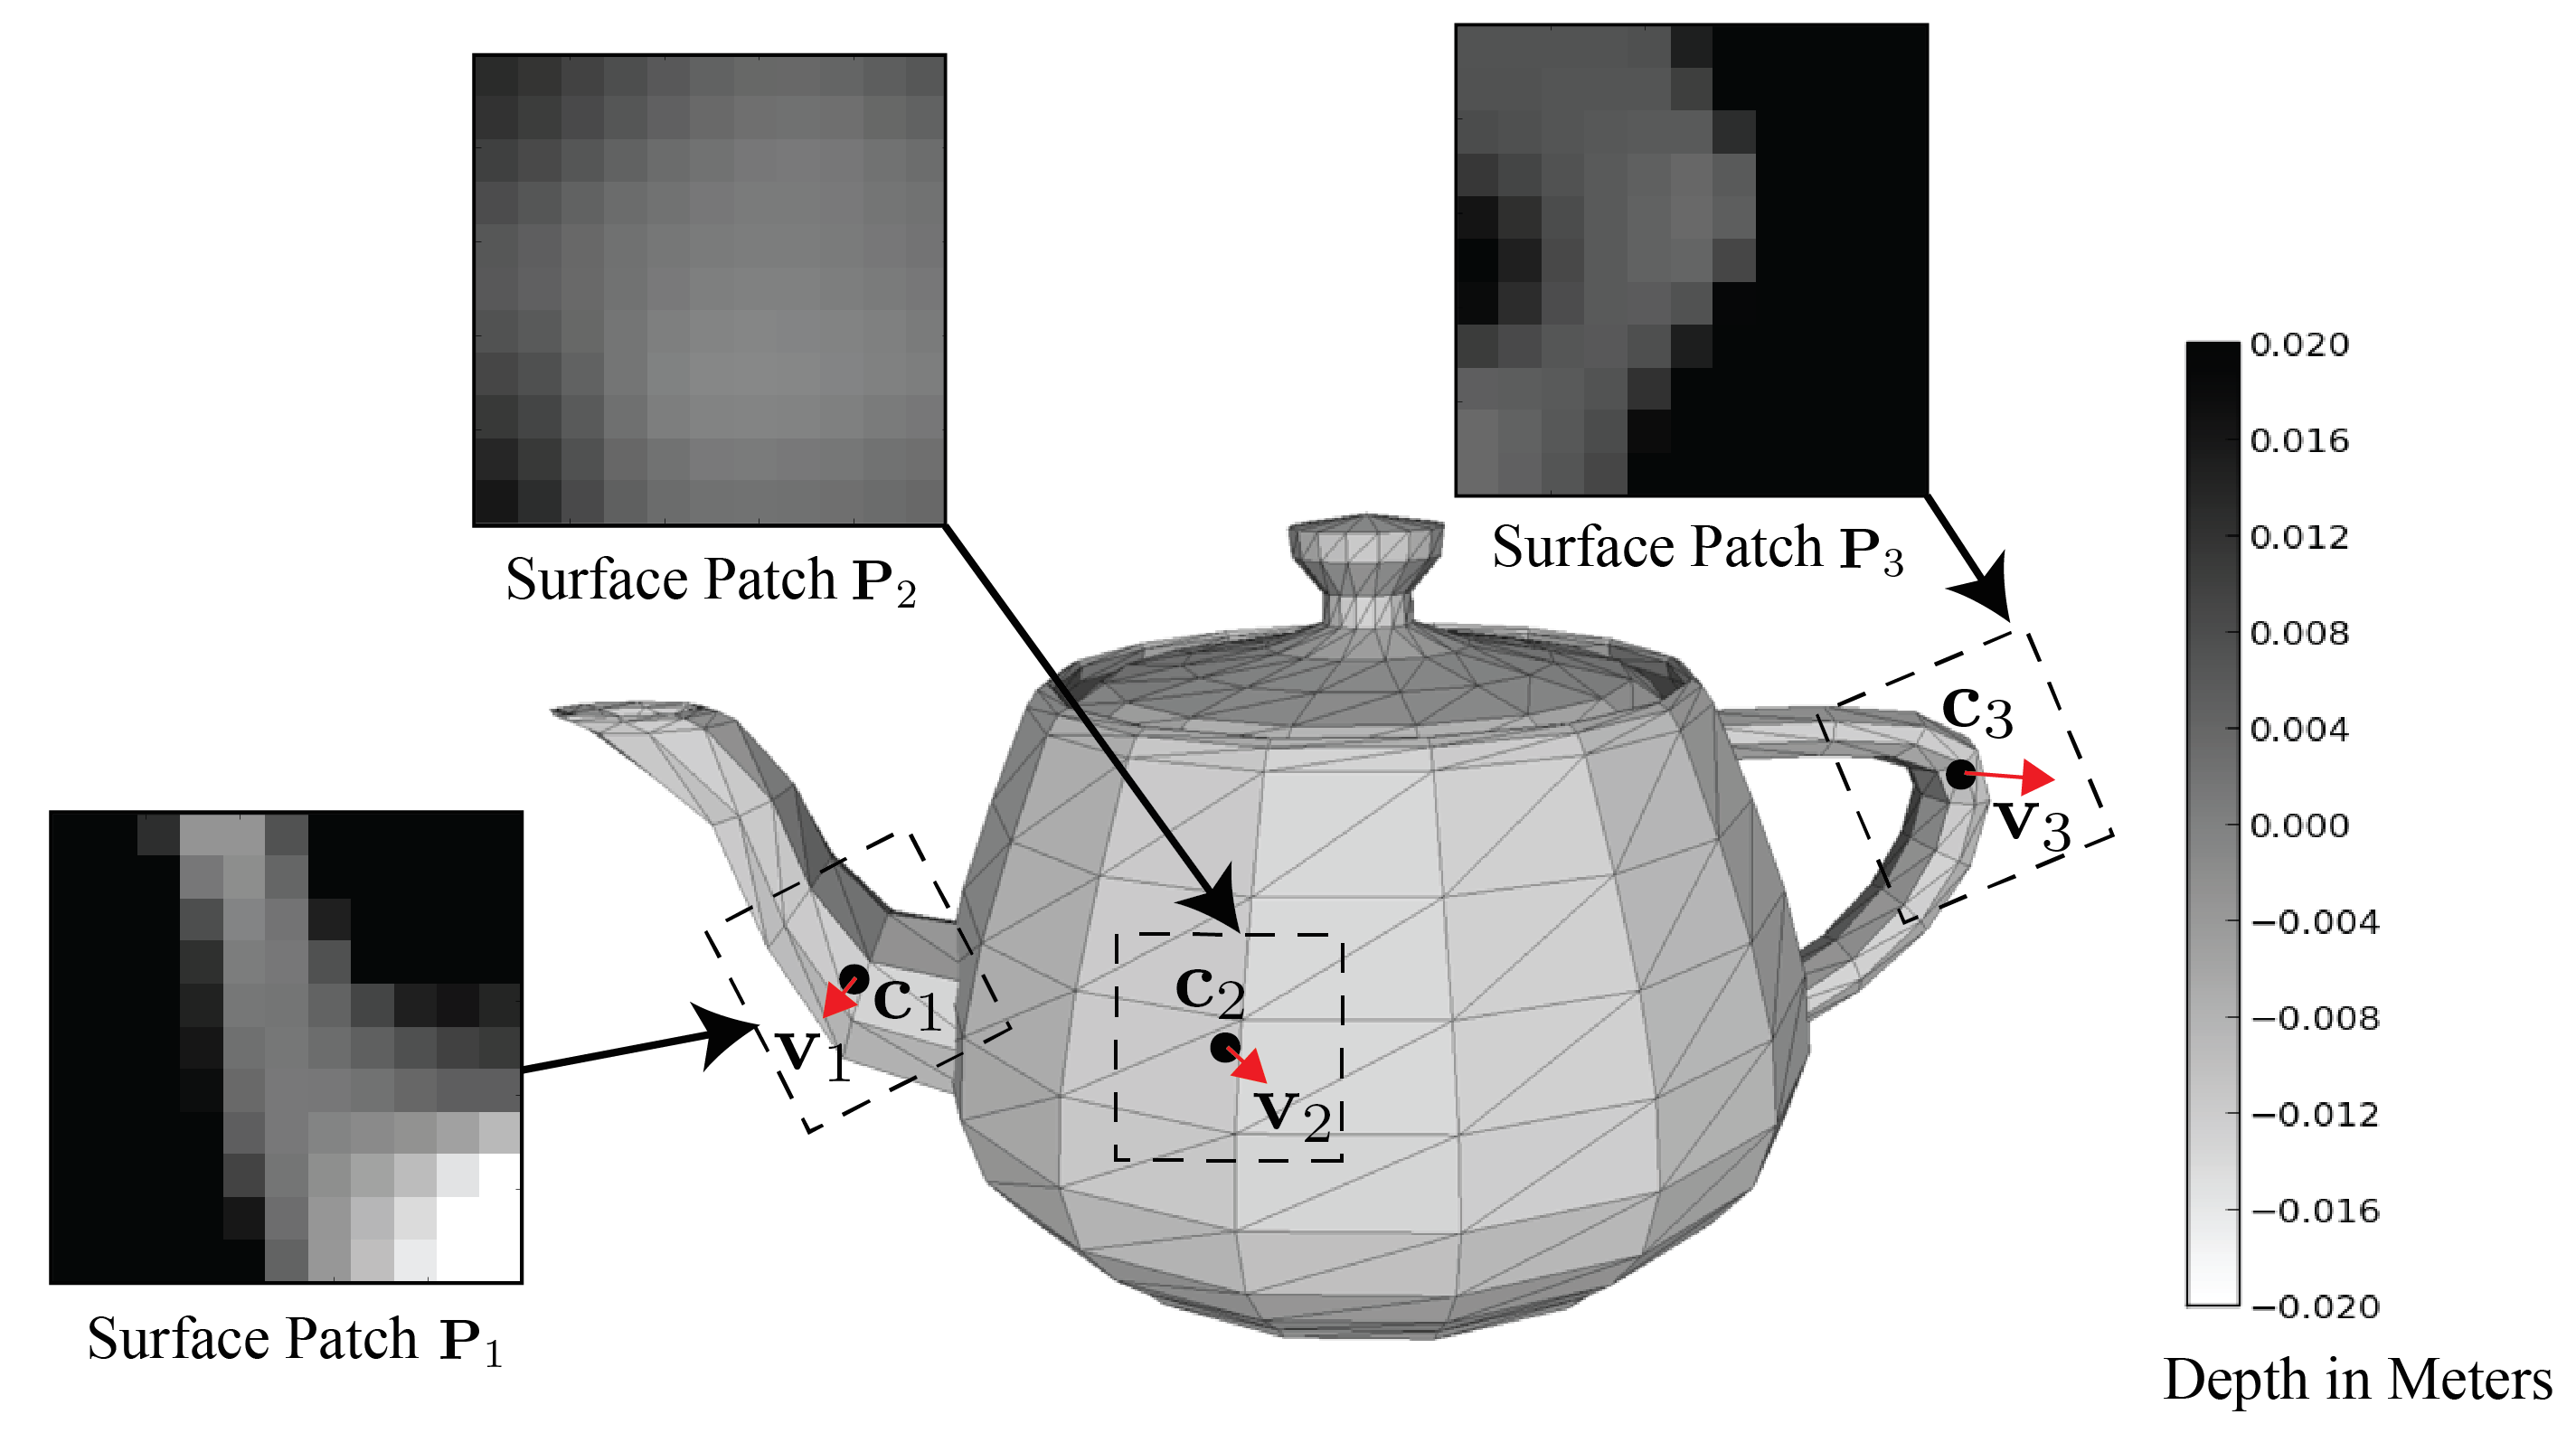
\includegraphics[scale=0.35]{figures/illustrations/local_feature_model.png}
%\caption{Three local surface heightmaps extracted on a teapot. Each heightmap is ``rendered" along the grasp axis at each contact point and oriented by the local directions of maximum variation in the heightmap.  We extract the gradients of these heightmaps as features in our robust grasp planning algorithm.}
%\figlabel{local-feature-model}
%\vspace*{-15pt}
%\end{figure}
%
%\subsubsection{Shape Features}
%\seclabel{global-sim}
%While force closure is based on local surface properties of an object around contact points, measuring global similarity may be useful because the heightmap gradients may not capture all possible contact locations for a grasp under perturbations in object and gripper pose.
%Thus we also use the feature map $\phi_{s}(\mY) = \psi(\mO)$, where $\psi$ is the similarity embedding based on MV-CNNs described in \secref{object-similarity}.

%\subsection{Thompson Sampling}
%\seclabel{thompson}
%
%Following Laskey et al.~\cite{laskey2015bandits}, we use Thompson sampling to select the next grasp to evaluate given belief distributions on the $P_F$ for each grasp on iteration $t$ specified by estimates $\mA_t = \{\alpha_{1,t}, ..., \alpha_{K,t}\}$ and $\mB_t = \{\beta_{1,t}, ..., \beta_{K,t}\}$.
%Thompson sampling samples a probability of force closure $\hat{\theta}_{j,t} \sim B(\alpha_{j,t}, \beta_{j,t})$ for all grasps $j = 1, ..., K$, then selects the grasp $j_t^* = \myargmax{j} \hat{\theta}_{j,t}$ to evaluate next.
%Several other criteria exist for selecting the next evaluation in MAB, such as Gittins indices~\cite{laskey2015bandits}, Upper Confidence Bounds~\cite{boularias2015learning}, and Expected Improvement~\cite{montesano2012active}.
 
